\documentclass[aps,prd,amssymb,amsmath,amsfonts,superscriptaddress,
floatfix ,preprintnumbers,altaffilletter]{revtex4}

\usepackage{epsfig}
\usepackage{graphics}
\usepackage{graphicx}
\usepackage{amsmath,amssymb,mathrsfs}
\usepackage{amsfonts}
\usepackage{color}
\usepackage{wasysym}
\usepackage{times}
\usepackage{mathptmx}
\usepackage{gensymb}
%\usepackage{fullpage}
\usepackage{appendix}
%\usepackage{fontenc}
\usepackage{listings}
%\usepackage[utf8]{inputenc}
%\usepackage{authblk}

%%%%%Some new commands%%%%%%%%%%%%%%%%%
\newcommand{\patricia}[1]{\textcolor{blue}{\textit{Patricia: #1}}}
\newcommand{\ian}[1]{\textcolor{blue}{\textit{Ian: #1}}}

\newcommand{\AEI}{Max Planck Institute for Gravitational Physics (Albert-Einstein-Institute), Am M\"uhlenberg 1, Potsdam-Golm, 14476, Germany}
\newcommand{\Ligo}{LIGO Laboratory, California Institute of Technology, MS 100-36, Pasadena, California 91125, USA}
\newcommand{\TAPIR}{Theoretical Astrophysics, Walter Burke Institute for Theoretical Physics, California Institute of Technology, Pasadena, California 91125, USA}
%%%%%%%%%%%%%%%%%%%%%%%%%%%%%%%%%

%%%%%%%%%%
\begin{document}
%%%%%%%%%%

\title{Numerical Relativity Injection Infrastructure}

\author{Patricia Schmidt}
\affiliation{\Ligo}
\affiliation{\TAPIR}

\author{Ian W. Harry}
\affiliation{\AEI}

\date{\today}

\begin{flushright}
LIGO-T1500606-v1
\end{flushright}

%%%%%%%%%%%%%%%
\begin{abstract}
\label{sec:abs}
%%%%%%%%%%%%%%%
This technical LIGO document describes the new standardised infrastructure in the LIGO Algorithms Library (LAL), 
which henceforth allows for the usage of Numerical Relativity (NR) waveforms as a discrete waveform approximant
in LIGO data analysis via the regular interfaces.
\end{abstract}

%%%%%%%%%%%%%%%
\maketitle 

%%%%%%%%%%%%%%%
\section{Introduction}
\label{sec:intro}
%%%%%%%%%%%%%%%
Gravitational waveforms from coalescing compact binary systems play a critical role in LIGO data analysis.
Whilst for low-mass systems only the early part of the inspiral is accessible to LIGO, for high-mass systems 
also the later stages of the binary evolution, in particular the merger and final ringdown, are visible in the LIGO
sensitivity band. 

Whilst the waveforms during the early part of the binary coalescence are accurately described by an
analytic post-Newtonian expansion of the Einstein field equations, the final stages require the full non-linear solution
of the field equations. So far, NR merger waveforms have predominantly been used to calibrate analytic waveform models
and to test those models against independent NR waveforms not used in the construction~\cite{}. 

However, in the advanced detector era, we may wish to directly use NR waveforms in gravitational-wave searches
and parameter estimation to test General Relativity and to assess the systematics of analytic waveforms models within
a uniform framework. To do so, we have recently developed a simple infrastructure to allow for the treatment of
NR waveforms as a ``discrete'' waveform approximant provided the NR data are available in a specific format. 
This allows the easy integration of NR waveforms into already existing data analysis pipelines.

Previously, hybrid waveforms of binary black holes constructed by combining a PN inspiral with an NR merger-ringdown 
waveform have been
used in LIGO data analysis and parameter estimation in the NINJA and NINJA-2 projects~\cite{Aylott:2009ya, Aasi:2014tra}.
This required the
NR waveforms to be resampled at uniform times \textbf{before} inserting the mass scale, whereas the new infrastructure uses a highly
compressed data format to represent the NR data. Additionally, 1D spline interpolants are used to allow for the resampling
of the waveforms \textbf{after} the mass scale has been inserted, which avoids the storage of large data sets.
The new injection infrastructure is designed to supercede and replace the previous method.

The remainder of this technical document is organised as follows: In Sec. \ref{sec:format} we give a brief introduction
to the format of the NR waveform data. In Sec. \ref{sec:gen} we describe the code basics and how NR waveforms
are generated in LAL/pyCBC. We highlight caveats and desired future improvements in Sec.~\ref{sec:discussion}.

%%%%%%%%%%%%%%%
\section{Waveform Format}
\label{sec:format}
%%%%%%%%%%%%%%%
In a Numerical Relativity simulation, one solves for the complete space-time of the binary system. For data analysis
purposes however, one requires the gravitational-wave strain $h(t)$ far from the source. The relevant numerical quantity
is the metric perturbation $h^{TT}_{ij}$ as computed in the transverse-traceless gauge (TT). 

There are different way of computing the metric perturbation from a numerical evolution. The most common methods include
the use of the complex Weyl scalar $\Psi_4$, which is related to the metric perturbation via two time derivatives, or the
Regge-Wheeler-Zerilli formalism computes the metric perturbation in the wave-zone as a perturbation of the Schwarzschild
spacetime. 

In the TT gauge, the metric perturbation
has two independent real polarisations, $h_+$ and $h_\times$, which can be written as a complex strain by
\begin{equation}
\label{ }
h = h_+ - i h_\times \in \mathbb{C},
\end{equation}
where $h_+, h_\times \in \mathbb{R}$.

Let $(t,x,y,z)$ be a Cartesian coordinate system in the wave-zone, which is related to the polar coordinates $(r, \theta, \phi)$ by the standard means. 
In this coordinate system, the metric perturbation is commonly decomposed into modes
in a basis of spin-weighted spherical harmonics, ${}^{-2}Y_{\ell m}$, of spin weight $s=-2$, where the GW propagation direction is
the radial unit vector r.
For any point $(\theta, \phi)$ on the unit sphere, the GW strain can then be shown to take the following form:
\begin{equation}
\label{ }
h(t; \theta, \phi) = h_+ - i h_\times = \sum_{\ell=2}^\infty \sum_{m=-\ell}^{\ell} h_{\ell m}(t) {}^{-2}Y_{\ell m}(\theta,\phi).
\end{equation}

As for any wave, we can also write each gravitational-wave mode $h_{\ell m}$ as an amplitude $A_{\ell m}$ and a phase
$\Phi_{\ell m}$,
\begin{equation}
\label{ }
h_{\ell m}(t) = A_{\ell m}(t)e^{i\Phi_{\ell m}(t)}.
\end{equation}
The amplitude of each mode is its complex norm, the phase is the unwrapped argument of the complex time series $h_{\ell m}$. 

%%%%%%%%%%%%%%%
\subsection{Spline Compression}
\label{sec:spline}
%%%%%%%%%%%%%%%
Gravitational waveforms for LIGO data analysis purposes require uniform sampling in time for a given sampling frequency $f_s$.
NR datasets however, are commonly not uniformly sampled and if they are, the sampling interval $dt$ may not necessarily
correspond to the one required by the data analysis code. It is therefore unavoidable to interpolate the NR data such that for any total
mass M and sampling rate the NR waveforms can be resampled accordingly. Whilst the NR data could simply be interpolated as
they are, we choose to reduce the data load and therefore also the I/O time by performing 1D spline compressions on the NR data~\cite{Galley:2015aa}. This is a particular advantage for long simulations or hybrid data, but also reduces the storage needed for pure NR data. \\

The 1D spline compression is performed separately for each mode amplitude $A_{\ell m}$ and phase $\Phi_{\ell m}$. The compression is
achieved by applying a greedy algorithm to the NR data, which selects the near-optimal points to construct a univariate spline interpolant
with a specified global accuracy. By default, the interpolants are constructed using fifth degree polynomials and a tolerance of $10^{-6}$,
i.e. if the spline is evaluated at the discrete times $t_i$ of the NR data, the original NR values are recovered with an error smaller than the
specified tolerance. For a detailed description of this method and the accuracy of the obtained interpolants, we refer the reader to~\cite{}. 
To perform the spline compression, the publicly available python package ``romSpline'' by Chad R. Galley is used~\cite{}. \\

Once the spline interpolants have been obtained, they are stored as individual groups in a single HDF5 file with the following group naming
conventions: 
\begin{itemize}
  \item Amplitude group: \textbf{amp\textunderscore l\#1\textunderscore m\#2}
  \item Phase group: \textbf{phase\textunderscore  l\#1\textunderscore m\#2},
\end{itemize}
where (\#1, \#2) are placeholders for $(\ell, m)$, e.g., for $(\ell=2, m=-2)$ the naming convention is phase\textunderscore l2\textunderscore m-2 and 
amp\textunderscore l2\textunderscore m-2. \\
\\We note that for NR data without a hybridised PN inspiral, the initial \emph{junk radiation} needs to be removed \textbf{before} the spline interpolants are constructed. 
Following the LAL waveform convention, the waveforms also need to be aligned such that the peak of the waveform occurs at $t_\mathrm{peak}=0$ 
before constructing the interpolants.


%%%%%%%%%%%%%%%
\subsection{Metadata}
\label{sec:meta}
%%%%%%%%%%%%%%%
The metadata format is adapted from the original NINJA-2 metadata format~\cite{Brown:2007jx}. For NINJA-2, the metadata were stored
additional text files. Any such file may still be included in the HDF5 files, but crucially 
each HDF5 has to include a \emph{minimal} set of metadata associated with the NR simulation stored as attributes of the HDF5 file. Currently, metadata for time-dependent physical quantities like the spin components are given for the time corresponding to the very first data point in the mode data stored in the HDF5 file, which we henceforth will refer to as the \emph{beginning} of the waveform. 

Further, the spin measurements \emph{and} the orbital phase at the beginning of the waveform have to be provided as measured in a very specific binary source frame, namely in one where the instantaneous orbital plane
defines the xy-plane and $\hat{L}$ points along the z-axis (see Fig.~\ref{fig:source} for an illustration). Note that this may involve some transformation of spin data depending on the NR code. However, the waveform data are unchanged.

More metadata can be added as desired but the minimal requirements are the following: \\
\begin{itemize}
\item {[}NR-group{]}: a string to identify the NR group/code
\item {[}type{]}: a brief description of the simulation, e.g. aligned-spins, precessing etc.
\item{[}name{]}: list here alternative names or internal identifiers of the simulation
\item{[}eta{]}: the symmetric mass ratio of the binary system
\item{[}f\textunderscore lower\textunderscore at\textunderscore 1MSUN{]}: frequency of the $(2,2)$-mode in Hz at the beginning of the waveform scaled to 1 solar mass
\item{[}coa\textunderscore phase{]}: this is twice the orbital reference phase at the beginning of the waveform
\item{[}spin1x{]}, {[}spin1y{]}, {[}spin1z{]}: spin components of the spin on the larger object measured w.r.t. to the orbital angular momentum L at the beginning of the waveform
\item{[}spin2x{]}, {[}spin2y{]}, {[}spin2z{]}: spin components of the spin on the smaller object measured w.r.t. to the orbital angular momentum L at the beginning of the waveform
\end{itemize}
To reduce potential ambiguities and to enable the usage of waveforms from matter simulations, we further recommend adding the following  additional metadata:
\begin{itemize}
\item{[}object1{]}, {[}object2{]}: a string to identify the object type, e.g. black hole, neutron star
\item{[}mass1{]}, {[}mass2{]}: matter simulations have a mass scale, hence not only the mass ratio but also the individual masses need to be accessible
\item{[}eccentricity{]}: eccentricity parameter of the simulation
%\item{[}NR\textunderscore frame{]}: the coordinate system , e.g. inertial, J-aligned etc.
\item{[}J\textunderscore hat{]}: the direction of the total angular momentum at the beginning of the waveform
\item{[}L\textunderscore hat{]}: the direction of the orbital angular momentum at the beginning of the waveform
\item{[}PN\textunderscore approximant{]}: string identifier for the inspiral if hybrid data are stored
\end{itemize}
For complete reproducibility and transparency, we recommend to store any NR metadata files and the original NR times $t_i$ as a datasets in the HDF5 file.

%%%%%%%%%%%%%%%
\section{Generating NR waveforms}
\label{sec:gen}
%%%%%%%%%%%%%%%
Once the HDF5 file has been provided, the NR waveforms can be generated through the standard waveform interfaces \texttt{ChooseTDWaveform()} in LAL
and \texttt{get\textunderscore td\textunderscore waveform()} in pyCBC~\cite{Canton:2014ena}. The lal approximant name is ``NR\textunderscore hdf5''. To call the test verification code in pycbc, specify the approximant ``NR\textunderscore hdf5\textunderscore pycbc''. 
As opposed to continuous approximants, the spline data are read from file and evaluated for the desired extrinsic
parameters. The intrinsic parameters in NR simulations are fixed, currently internal checks on the mass ratio and the spin components 
are performed to guarantee the consistency between the values passed
in the waveform generation call and metadata values. \\
\\For a given starting frequency and total mass, a time array is allocated based on an estimate of the waveform length. We use the LAL function 
\texttt{SimIMRSEOBNRv2ChirpTimeSingleSpin()} to estimate the waveform length with an additional leverage of 10\%. If the NR waveforms are not long
enough, the generation is aborted. From the estimated length and the desired sampling rate, the discrete time series for the spline evaluation is
determined.

To construct the polarisation $h_+$ and $h_\times$, the splines for each amplitude and phase are evaluated at the points in the discrete time times, 
weighted by the ${}^{-2}Y_{lm}$, and summed up:
\begin{align}
\label{}
    \mathrm{Re}(h_{\ell m}) &= A_{\ell m} \cos(\Phi_{\ell m}),   \\
    \mathrm{Im}(h_{\ell m}) &= A_{\ell m} \sin(\Phi_{\ell m}),   \\
    h_+ &= \sum_{\ell, m} \mathrm{Re}(h_{\ell m}) \mathrm{Re}({}^{-2}Y_{\ell m}) + \mathrm{Im}(h_{\ell m}) \mathrm{Im}({}^{-2}Y_{\ell m}), \\
    h_\times &= \sum_{\ell, m} \mathrm{Re}(h_{\ell m}) \mathrm{Im}({}^{-2}Y_{\ell m}) - \mathrm{Im}(h_{\ell m}) \mathrm{Re}({}^{-2}Y_{\ell m}),
\end{align}
where the polar angle $\theta$ denotes the angle between the orbital angular momentum and the line-of-sight and the azimuthal
angle $\phi$ is the sum of parameter value 'coa\textunderscore phase' and any reference phase passed in the waveform generator function.
\\
Note that all waveform modes $(\ell, m)$ contained in the HDF5 file are used
to compute the two polarisations. The algorithm will incorporate any mode between $\ell =2$ and $\ell =8$ if present in the
HDF5 file but at least the $(\ell=2, m=2)$ has to be present in the NR data file. \\
\\
The compressed NR data files do not store the splines themselves, but the knots, errors, the polynomial degree etc. In the pyCBC implementation,
the splines are constructed from the HDF5 file via the python function \texttt{UnivariateSpline}, in the LAL implementation regular GSL interpolation
is performed. Fig.~\ref{fig:waveforms} shows an example comparison between NR waveforms obtained using the pyCBC and the LAL waveform generators. The mismatch
between the waveforms is less than $10^{-7}$. This is consistent with the level of disagreement expected due to the different numerical interpolation
routines. \\
The source codes can be found in \texttt{lalsuite/lalsimulation/src/LALSimIMRNRWaveforms.c} and 
\texttt{pycbc/pycbc/waveforms/nr\textunderscore waveform.py} respectively.

%%%%%%%%%%
\subsection{Examples}
%%%%%%%%%%
There are a variety of different ways to generate waveforms using LIGO data analysis software. Here, we give two specific examples
for function calls in python, firstly directly via the pyCBC implementation, and secondly through the SWIG-wrapped version of 
lalsimulation. 

\begin{enumerate}
  \item The pyCBC implementation of the waveform generator may be called in the following way through python: \\
\begin{lstlisting}
from pycbc.waveform import get_td_waveform 

hp, hc = get_td_waveform(approximant='NR_hdf5', 
                         numrel_data='/PATH/TO/HDF5',
                         mass1, mass2,
                         spin1x, spin1y, spin1z,
                         spin2x, spin2y, spin2z, 
                         delta_t, f_lower, f_ref,
                         inclination, distance, 
                         coa_phase)
\end{lstlisting}

\item To use the implementation in LALSimulation through SWIG, use the following function call in python:\\
\begin{lstlisting}[mathescape=true]
import lalsimulation as lalsim

flags = lalsim.SimInspiralCreateWaveformFlags()

lalsim.SimInspiralSetNumrelData(flags,'/PATH/TO/HDF5')

hp, hc = lalsim.SimInspiralChooseTDWaveform(phiRef, 
              deltaT, m1 * MSUN_SI, m2 * MSUN_SI, 
              s1x, s1y, s1z,
              s2x, s2y, s2z, 
              fStart, fRef, 
              distance, inclination,
              $\lambda_1=0$, $\lambda_2=0$, 
              flags, nonGRparams=None, 
              amplitudeO=-1, phaseO=-1, 
              approximant=lalsim.NR_hdf5),
\end{lstlisting}
where $\lambda_1$ denote the tidal deformation parameters, which vanish in the case of black holes. 
\end{enumerate}
Fig.~\ref{fig:waveforms} shows the two waveform polarizations $h_+$ and $h_{\times}$ for the binary black hole hole case simulated in case 
SXS:BBH:0019 from the publicly available SXS catalogue~\cite{Mroue:2013xna} for a total mass of 50 $\mathrm{M}_\odot$. The dimensionless spins for this simulation are
$\vec{\chi}_1=(0,0,-0.5)$ and $\vec{\chi}_2=(0,0,0.499)$ and the component masses are $m_1=30.01360$ and $m_2=20.00954$.
As extrinsic parameters, we choose the following: distance=100Mpc, inclination=0.4rad, deltaT=1.0/16384, fStart=fRef=18.88Hz. We do not alter
the reference phase but instead pass the metadata value stored in the HDF5 file. We have obtained those polarizations via the lalsimulation interface and also via the test verification code in pycbc. The match between the waveforms obtained from the two numerical implementations is $\mathcal{M}=0.999999999341$.
\begin{figure}
\begin{center}
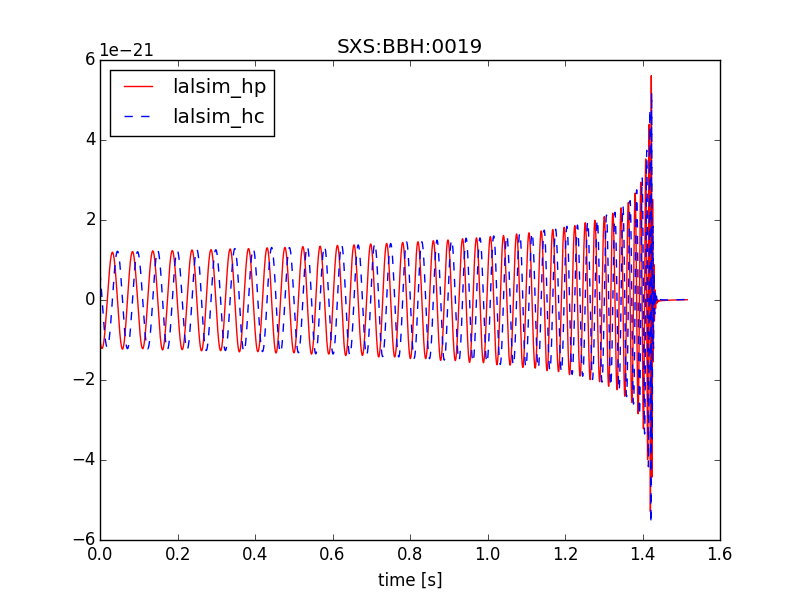
\includegraphics[width=80mm]{lalsim_TD_0019.png}
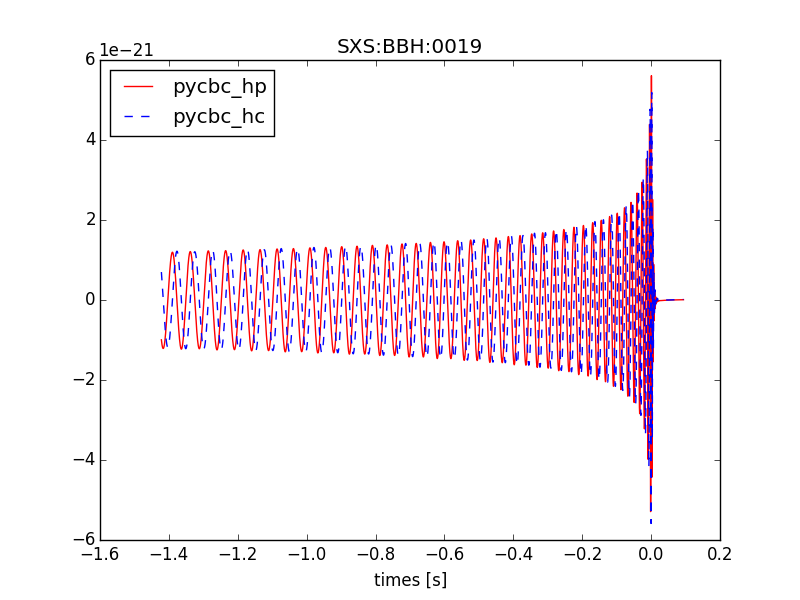
\includegraphics[width=80mm]{pycbc_TD_0019.png}
\caption{The waveform polarizations $h_+$(solid, red) and $h_\times$(dashed, blue) of the publicly available SXS waveform SXS:BBH:0019 
generated via the waveform interface in lalsimulation (left panel) and in pyCBC (right panel).}
\label{fig:waveforms}
\end{center}
\end{figure}


%%%%%%%%%%
\section{Discussion}
\label{sec:discussion}
%%%%%%%%%%

With this new infrastructure it should be much easier, and much less memory intensive, to use NR waveforms
directly for data-analysis applications. The ``NR\_hdf5'' approximant works much the same as any other approximants
in lalsimulation, but does have a few important differences. The user must supply the location of the HDF file
corresponding to the waveform to be injected, this functionality was already available from NINJA, but was not
previously used in lalsimulation. Second the user must be careful to supply mass ratio and spin values that
are consistent with the NR files. Small changes are therefore needed to use this approximant in applications
and we will be happy to assist with implementing such changes. PyCBC and lalinference already have test branches
where this is available.

There are also still a few caveats to the current implementation, which we plan to investigate with the waveform review committee.
As opposed to the continuous waveform approximants, at the moment the metadata
are only referring to the beginning of the waveform and not some reference time, which can be chosen freely. While this is 
not a problem for aligned-spin binaries, this poses a rather big problem for precessing simulations. To fully integrate this
desired freedom, additional information needs to be incorporated into the HDF5 files and the waveform generator
accordingly. In particular, the relevant information would have to include the spins as a function of frequency as well
as the orbital angular momentum direction. 

%%%%%%%%%%%%%%%%%%%%%%%%%Acknowledgements%%%%%%%%%%%%%%%%%%%%
\section*{Acknowledgments}
We thank Kent Blackburn for carefully reading through the manuscript and providing useful comments.

%%%%%%%%%%%%%%%%%%%%%%%%%Appendices%%%%%%%%%%%%%%%%%%%%%%%%
\appendix
%%%%%%%%%
\section{Conventions and frame choices}
\label{sec:conv}
%%%%%%%%%%
The new infrastructure provides a standardised interface between NR and LIGO data analysis. To guarantee
the correct waveform handling, in particular for precessing binary simulations, certain conventions and frame
choices must be considered. 

The current setup is as follows: At the start of the waveform, i.e. the first entry in the NR time series considered in the
HDF5 file, the instantaneous orbital plane, characterized by its orthonormal direction $\hat{L}$, has some (arbitrary) orientation
in the Cartesian simulation frame $(x, y, z)$ of the NR simulation. The polar angle between the line-of-sight $\hat{N}$ and the instantaneous orbital angular momentum direction is denoted as $\theta$ and corresponds to the option parameter ``inclination'' in the waveform generator functions. 

If the NR simulation the frame is defined such that $\hat{L}$ does not point along the z-axis at the start of the waveform, the additional angle between $\hat{L}$ and the z-axis needs to be taken into account when setting the value for the inclination parameter. Currently, it is up to the user to take care of this, but we aim to integrate this into the waveform generator. 

The azimuthal angle $\phi$ denotes the instantaneous orientation of the orbital separation at the beginning of the waveform in the source frame, where $\hat{L}$ points along the z-axis. The metadata parameter ``coa\textunderscore phase'' is twice this angle.

\begin{figure}[!h]
\begin{center}
\def\svgwidth{0.4\columnwidth}
\input{SourceFrame.pdf_tex}
\caption{Binary source frame for spin and orbital phase measurements: The spins and orbital phase measurements at the
beginning of the NR data set have to be provided in a frame, where $\hat{L}$ points along the z-direction.}  
\label{fig:source}
\end{center}
\end{figure}

%%%%%References%%%%%%%%%%%%%%%%%

\bibliography{nrinj}

%%%%%%%%%%
\end{document}
%%%%%%%%%%
